% ==========================================================================
\chapter{数值验证}
% ==========================================================================

本章用数值实验检验第四章的理论预测。第 \ref{sec:exp-design} 节说明实验设计与误差度量；第 \ref{sec:stiff-map} 节给出刚性相图；第 \ref{sec:max-dt} 节比较最大稳定步长；第 \ref{sec:shock-accuracy} 节定量分析激波精度；第 \ref{sec:convergence} 节验证网格收敛性；第 \ref{sec:exp-discussion} 节讨论稳定性与精度的关系。

\section{实验设计}
\label{sec:exp-design}

所有实验均基于第三章的有限体积半离散格式与 IMEX-Euler 时间推进。代码以 Python 实现，空间算子采用一阶 Rusanov 通量（稳定性实验）或 MUSCL/minmod 重构（精度实验），时间推进使用固定步长的 IMEX-Euler。线性系统用稀疏 LU 分解求解，矩阵在步长固定时只分解一次。

实验分为四组，分别回答四个问题：
\begin{enumerate}[label=(\arabic*),leftmargin=2.4em]
  \item 固定 CFL、扫描 $\nu$ 与 $\theta$，稳定性区域是否与 $\theta\le1/2$ 的预测一致？
  \item 固定 $\nu$、扫描 $\theta$，最大稳定步长如何随 $\theta$ 变化？是否与定理 \ref{thm:main} 及离散条件 \eqref{eq:sawtooth-condition} 一致？
  \item 在稳定的参数下，不同 $\theta$ 对激波位置、过渡层厚度和 $L^1$ 误差有何影响？
  \item 空间网格加密时，格式的观测收敛阶是多少？
\end{enumerate}

误差度量定义如下。设数值解为 $u_j$，精确解为 $u_{\rm ex}(x_j,t)$，定义平均 $L^1$ 误差
\begin{equation}
  E_1=\frac{1}{|\Omega|}\int_\Omega|u-u_{\rm ex}|\,\dd x,
  \label{eq:L1-error}
\end{equation}
用梯形公式计算。激波位置 $x_s$ 定义为 $u=0.5$ 的等值点，用线性插值确定；过渡层厚度 $w$ 定义为 $u=0.9$ 与 $u=0.1$ 两个等值点之间的距离。精确解的对应量为 $x_s^{\rm ex}=st$ 与 $w_{\rm ex}=4\nu\ln9/A$。

稳定性判据采用两种方式。对线性分析，直接计算所有 Fourier 模态的放大因子，若 $\max_\xi|R(\xi)|\le1$ 则判定稳定。对稳定性实验中的非线性计算，若解的最大模超过 $0.55$（约为初始最大模 $0.5$ 的 $1.1$ 倍）或出现非有限值，则判定失稳。

\section{刚性相图}
\label{sec:stiff-map}

第一组实验固定 $N=200$、$\Delta t=0.4\Delta x$、$t=1$，在周期区间 $[0,1]$ 上取初始条件
\begin{equation}
  u_0(x)=0.5+0.01\sin(2\pi x),
  \label{eq:smooth-ic}
\end{equation}
扫描 $\nu\in[10^{-2},10^{2}]$（对数网格，21 个点）与 $\theta\in[0,1]$（41 个点），记录终时刻的 $\max|u|$。稳定时 $\max|u|\approx0.5$；失稳时该值迅速增大。结果画成 $(\theta,\log_{10}\nu)$ 平面上的热图，颜色表示 $\log_{10}\max|u|$。

\begin{figure}[htbp]
  \centering
  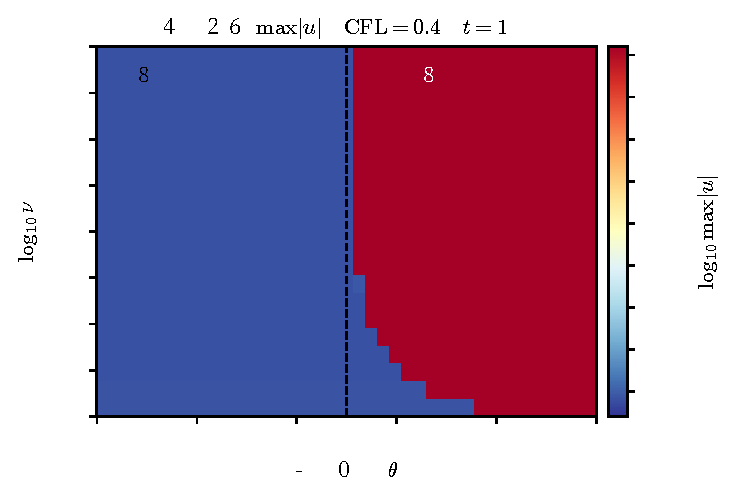
\includegraphics[width=0.74\textwidth]{stiff_heatmap.pdf}
  \caption{刚性相图：固定 $\CFL=0.4$、$N=200$、$t=1$，扫描 $\theta$ 与 $\nu$。颜色为 $\log_{10}\max|u|$；虚线为 $\theta=1/2$。}
  \label{fig:stiff-map}
\end{figure}

图 \ref{fig:stiff-map} 显示了一个清晰的相变：$\theta\le1/2$ 的整个左半区域保持稳定（深蓝色），$\theta>1/2$ 的区域在 $\nu$ 较大时变为红色（失稳）。分界线与 $\theta=1/2$ 的竖直虚线高度吻合。具体而言：

\begin{itemize}[leftmargin=2.2em]
  \item $\theta=0$、$0.25$、$0.5$ 在所有测试的 $\nu$ 下都稳定，包括 $\nu=100$ 的强刚性情形；
  \item $\theta=0.55$ 时，$\nu\lesssim0.06$ 稳定，$\nu\gtrsim0.1$ 失稳；
  \item $\theta=0.6$ 时，阈值约为 $\nu\approx0.03$；
  \item $\theta=0.75$ 时，阈值约为 $\nu\approx0.0125$；
  \item $\theta=1$ 时，即使 $\nu=0.01$ 也已失稳，因为此时 $r=\nu\Delta t/\Delta x^2=0.8>1/2$，显式扩散本身就不稳定。
\end{itemize}

这些阈值可以用网格尺度条件 \eqref{eq:sawtooth-condition} 定量解释。在 $\xi=\pi$ 处，$c=\Delta t/\Delta x=0.4$，$r=\nu\Delta t/\Delta x^2=80\nu$（取 $\Delta x=0.005$）。由 $c+2(2\theta-1)r\le1$ 解出
\begin{equation}
  \nu\le\nu_{\max}=\frac{\Delta x^2}{2\Delta t(2\theta-1)}
  =\frac{6.25\times10^{-3}}{2\theta-1}.
  \label{eq:nu-max}
\end{equation}
对 $\theta=0.55$、$0.6$、$0.75$、$1$，分别得到 $\nu_{\max}=0.0625$、$0.03125$、$0.0125$、$0.00625$，与热图中的转变位置一致。这说明相图的边界不是数值偶然，而是由离散符号精确决定的。

\section{最大稳定步长}
\label{sec:max-dt}

第二组实验固定 $N=200$、$\nu=1$，在周期区间上取初始条件 \eqref{eq:smooth-ic}，并叠加一个幅度为 $10^{-8}$ 的网格尺度扰动 $(-1)^j$。这个种子是必要的：若初值完全光滑，网格尺度模态不会被激发，有限时间的二分法会高估稳定步长。对每个 $\theta$，用二分法寻找最大的稳定步长；每次试验固定推进 $20000$ 步，而不是固定物理终时，因为稳定性是每步性质。

线性预测通过扫描所有 $\xi\in[0,\pi]$、要求 $\max|R(\xi)|\le1$ 得到。图 \ref{fig:max-dt} 给出了 $\Delta t_{\max}$ 随 $\theta$ 的变化（对数纵轴）。曲线呈现出两个截然不同的区域：

\begin{figure}[htbp]
  \centering
  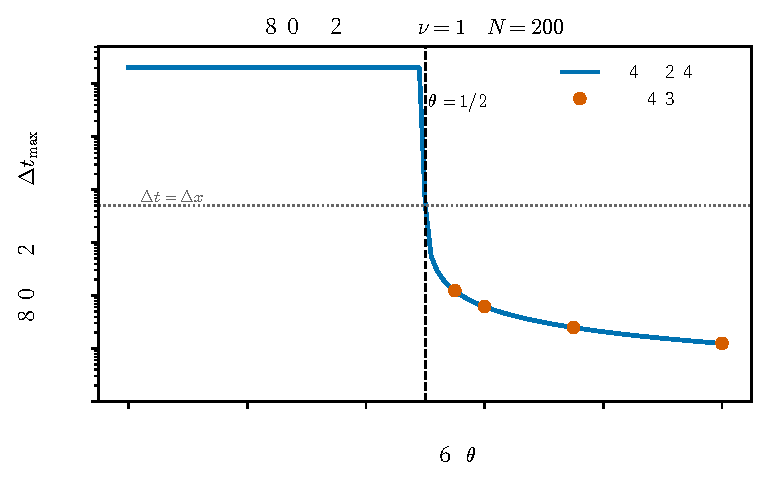
\includegraphics[width=0.74\textwidth]{maxdt.pdf}
  \caption{最大稳定步长随 $\theta$ 的变化（$\nu=1$，$N=200$，$\Delta x=0.005$）。实线为线性稳定性预测，圆点为非线性实验；虚线为 $\theta=1/2$。}
  \label{fig:max-dt}
\end{figure}

\begin{itemize}[leftmargin=2.2em]
  \item 当 $\theta<1/2$ 时，$\Delta t_{\max}$ 几乎不变，约为 $2.05$。此时稳定性由低波数扩散条件 \eqref{eq:low-k-numerical} 控制，而不是 CFL 条件。代入 $\nu=1$、$\Delta x=0.005$、$a=1$，得 $(2\nu+\Delta x)/a^2=2.005$，线性符号预测为 $2.056$，略高于渐近值，这是离散符号的修正。
  \item 当 $\theta=1/2$ 时，$\Delta t_{\max}$ 突然降到 $\Delta x=0.005$。此时网格尺度条件退化为 $c\le1$，即 $\Delta t\le\Delta x$；低波数条件虽然允许更大的步长，但 $c\le1$ 成为起决定作用的约束。
  \item 当 $\theta>1/2$ 时，$\Delta t_{\max}$ 按 $1/(2\theta-1)$ 衰减。由 \eqref{eq:sawtooth-condition} 得
  \begin{equation}
    \Delta t_{\max}=\frac{\Delta x^2}{2\nu(2\theta-1)}.
    \label{eq:dt-max-formula}
  \end{equation}
  对 $\theta=0.55,0.6,0.75,1$，实测值与线性符号预测分别相差 $1.6\%$、$0.8\%$、$0.3\%$、$0.2\%$；与渐近公式 \eqref{eq:dt-max-formula} 的差别更小。
\end{itemize}

表 \ref{tab:max-dt} 汇总了代表性结果。需要强调，$\theta=1/2$ 的“突然下降”并不是说格式在 $\theta=1/2$ 处不稳定；它仍然稳定，只是允许的步长从“扩散控制”切换到了“CFL 控制”。这一切换是最大步长曲线出现断崖的原因。

\begin{table}[htbp]
  \centering
  \caption{不同 $\theta$ 下的最大稳定步长（$\nu=1$，$N=200$，$\Delta x=0.005$）}
  \label{tab:max-dt}
  \begin{tabular}{ccccc}
    \toprule
    $\theta$ & 理论公式 \eqref{eq:dt-max-formula} & 线性符号预测 & 非线性实验 & 相对偏差 \\
    \midrule
    $0$     & 无（扩散控制） & $2.056$ & --- & --- \\
    $0.25$  & 无（扩散控制） & $2.030$ & --- & --- \\
    $0.5$   & $\Delta x=5.000\times10^{-3}$ & $5.000\times10^{-3}$ & --- & --- \\
    $0.55$  & $1.250\times10^{-4}$ & $1.220\times10^{-4}$ & $1.239\times10^{-4}$ & $1.6\%$ \\
    $0.6$   & $6.250\times10^{-5}$ & $6.173\times10^{-5}$ & $6.223\times10^{-5}$ & $0.8\%$ \\
    $0.75$  & $2.500\times10^{-5}$ & $2.488\times10^{-5}$ & $2.496\times10^{-5}$ & $0.3\%$ \\
    $1$     & $1.250\times10^{-5}$ & $1.247\times10^{-5}$ & $1.249\times10^{-5}$ & $0.2\%$ \\
    \bottomrule
  \end{tabular}
\end{table}

表中“相对偏差”以线性符号预测为基准。对 $\theta<1/2$，线性阈值来自长波条件 \eqref{eq:low-k-numerical}；在 $L=1$、$N=200$ 的周期域上，第一个离散波数 $k=2\pi$ 已经落在不稳定带之外，因此有限时间内观察不到失稳。对 $\theta=1/2$，最不稳定模态是网格尺度，但其增长率在临界点附近趋于零，$20000$ 步内不足以把 $10^{-8}$ 的种子放大到可测幅度。这两种情形的非线性实验记为“---”，以线性符号预测为准；$\theta\ge0.55$ 的实验点则与预测吻合到 $2\%$ 以内。

\section{激波精度}
\label{sec:shock-accuracy}

第三组实验在 $[-2,3]$ 上计算粘性激波，取 $\nu=0.01$、$u_L=1$、$u_R=0$、$t=2$，初始条件为精确解 \eqref{eq:exact-shock} 在 $t=0$ 的值。网格 $N=800$，$\Delta x=6.25\times10^{-3}$，$\CFL=0.2$。此时 $r=\nu\Delta t/\Delta x^2=0.32<1/2$，所有 $\theta$ 都稳定。分别用一阶 Rusanov 与 MUSCL/minmod 计算 $\theta=0,0.25,0.5,0.75,1$ 五组解。

\begin{figure}[htbp]
  \centering
  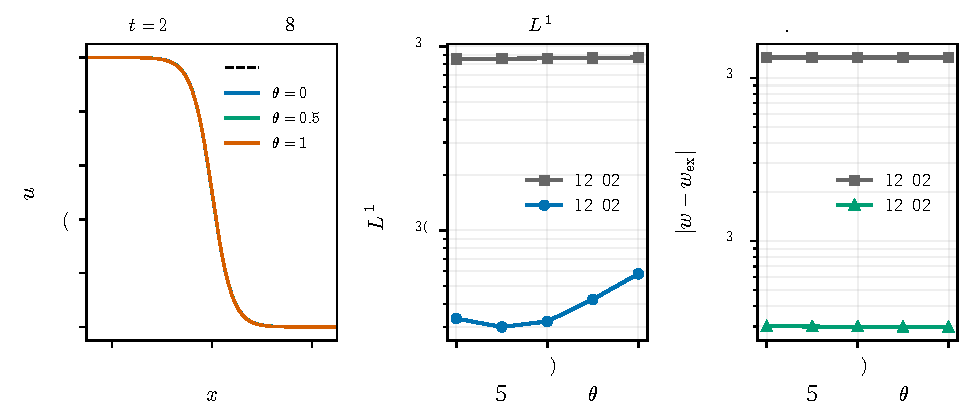
\includegraphics[width=0.98\textwidth]{shock_results.pdf}
  \caption{粘性激波的数值结果（$\nu=0.01$，$N=800$，$\CFL=0.2$，$t=2$）。(a) 剖面；(b) $L^1$ 误差随 $\theta$ 的变化；(c) 过渡层厚度误差随 $\theta$ 的变化。}
  \label{fig:shock-results}
\end{figure}

图 \ref{fig:shock-results}(a) 给出了 $\theta=0,0.5,1$ 的剖面与精确解。三条曲线在视觉上几乎重合，说明在稳定的参数下，$\theta$ 对整体波形的影响很小。差异体现在误差指标上。

\begin{table}[htbp]
  \centering
  \caption{激波算例的误差指标（$N=800$，$\nu=0.01$，$t=2$，$\CFL=0.2$）}
  \label{tab:shock-metrics}
  \small
  \begin{tabular}{ccccc}
    \toprule
    $\theta$ & \multicolumn{2}{c}{一阶 Rusanov} & \multicolumn{2}{c}{MUSCL/minmod} \\
    \cmidrule(lr){2-3}\cmidrule(lr){4-5}
     & $E_1$ & $|x_s-x_s^{\rm ex}|$ & $E_1$ & $|x_s-x_s^{\rm ex}|$ \\
    \midrule
    $0$    & $8.543\times10^{-4}$ & $1.395\times10^{-3}$ & $3.322\times10^{-5}$ & $1.041\times10^{-4}$ \\
    $0.25$ & $8.573\times10^{-4}$ & $1.477\times10^{-3}$ & $2.992\times10^{-5}$ & $8.40\times10^{-6}$ \\
    $0.5$  & $8.602\times10^{-4}$ & $1.560\times10^{-3}$ & $3.207\times10^{-5}$ & $8.73\times10^{-5}$ \\
    $0.75$ & $8.651\times10^{-4}$ & $1.642\times10^{-3}$ & $4.222\times10^{-5}$ & $1.831\times10^{-4}$ \\
    $1$    & $8.700\times10^{-4}$ & $1.725\times10^{-3}$ & $5.812\times10^{-5}$ & $2.788\times10^{-4}$ \\
    \bottomrule
  \end{tabular}
\end{table}

由表 \ref{tab:shock-metrics} 与图 \ref{fig:shock-results} 可以得到以下观察。

第一，一阶格式的误差主要由数值扩散主导。精确过渡层厚度为 $w_{\rm ex}=0.08789$，一阶格式给出 $w\approx0.10125$，相对误差约 $15.2\%$。这部分数值扩散来自 Rusanov 通量，其系数约为 $\Delta x/2=3.1\times10^{-3}$，远大于物理粘性 $\nu=0.01$ 的高波数贡献。不同 $\theta$ 的 $E_1$ 只相差约 $1.8\%$（从 $8.543\times10^{-4}$ 到 $8.700\times10^{-4}$），说明在一阶精度下，$\theta$ 的影响被空间误差掩盖。

第二，MUSCL 重构显著降低了误差。$E_1$ 从 $8.5\times10^{-4}$ 降到 $3.0\times10^{-5}$ 至 $5.8\times10^{-5}$，降低约 $15$ 至 $28$ 倍；过渡层厚度的误差从 $1.34\times10^{-2}$ 降到 $3.0\times10^{-4}$，降低约 $45$ 倍。这说明空间重构是提高精度的主要途径。

第三，在 MUSCL 格式中，$\theta$ 的影响变得可见，但不是单调的。$\theta=0.25$ 给出最小的 $E_1=2.992\times10^{-5}$ 与最小的位置误差 $8.4\times10^{-6}$；$\theta=0.5$ 次之（$3.207\times10^{-5}$），$\theta=0$ 第三（$3.322\times10^{-5}$）；$\theta=1$ 给出最大的 $E_1=5.812\times10^{-5}$，约为最优值的 $1.94$ 倍。这与“隐式越多越耗散”的直觉部分一致：$\theta=0$ 的隐式扩散最强，会增加一点数值耗散；$\theta=1$ 的显式扩散最弱，但会在激波附近留下轻微的振荡（$L^\infty$ 误差从 $2.50\times10^{-3}$ 增至 $4.34\times10^{-3}$）。$\theta=0.25$ 在两者之间取得了平衡。

第四，所有 $\theta$ 在 $\CFL=0.2$ 下都是稳定的，但稳定性边界并不相同。若把 $\CFL$ 提高到 $0.4$，$\theta=0.75$ 与 $1$ 会失稳（因为 $r=0.64>1/2$ 且 $c+r>1$），而 $\theta\le0.5$ 仍然稳定。因此，“哪个 $\theta$ 更准确”的比较必须在共同的稳定区域内进行；离开稳定区域，精度无从谈起。

\section{网格收敛性}
\label{sec:convergence}

第四组实验固定 $\nu=0.01$、$\CFL=0.2$、$t=1$，取 $N=100,200,400,800$，分别计算一阶格式（$\theta=0.5$）与 MUSCL 格式（$\theta=0,0.5$）的 $L^1$ 误差。结果如图 \ref{fig:convergence} 与表 \ref{tab:convergence} 所示。

\begin{figure}[htbp]
  \centering
  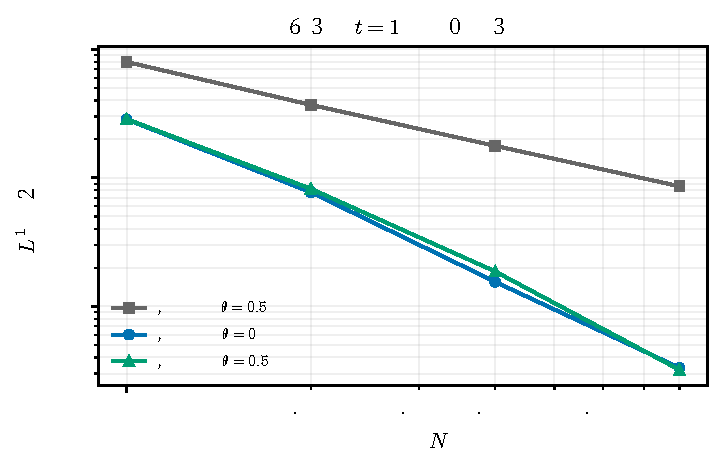
\includegraphics[width=0.72\textwidth]{convergence.pdf}
  \caption{网格收敛性（$\nu=0.01$，$\CFL=0.2$，$t=1$ 的移动粘性激波）。括号内为由首末两点估计的观测阶。}
  \label{fig:convergence}
\end{figure}

\begin{table}[htbp]
  \centering
  \caption{$L^1$ 误差随网格数的变化（$\nu=0.01$，$\CFL=0.2$，$t=1$）}
  \label{tab:convergence}
  \begin{tabular}{cccc}
    \toprule
    $N$ & 一阶，$\theta=0.5$ & MUSCL，$\theta=0$ & MUSCL，$\theta=0.5$ \\
    \midrule
    $100$ & $7.970\times10^{-3}$ & $2.854\times10^{-3}$ & $2.864\times10^{-3}$ \\
    $200$ & $3.692\times10^{-3}$ & $7.715\times10^{-4}$ & $8.213\times10^{-4}$ \\
    $400$ & $1.771\times10^{-3}$ & $1.551\times10^{-4}$ & $1.868\times10^{-4}$ \\
    $800$ & $8.588\times10^{-4}$ & $3.322\times10^{-5}$ & $3.207\times10^{-5}$ \\
    \midrule
    观测阶 & $1.07$ & $2.14$ & $2.16$ \\
    \bottomrule
  \end{tabular}
\end{table}

一阶格式的观测阶为 $1.07$，接近理论值 $1$。MUSCL 格式的观测阶为 $2.14$ 与 $2.16$，略高于 $2$。这一“超收敛”并不奇怪：本文的激波是粘性激波，过渡层是光滑的，且宽度约为 $14$ 个网格；minmod 限制器虽然会在极值点附近降低斜率，但在整个过渡层内解是单调的，重构基本保持二阶。若换成无粘激波（真正的间断），限制器会在间断处退化为一阶，观测阶通常会降到 $1$ 左右。因此，这里的二阶收敛是对“光滑粘性激波”而言的，不能直接推广到所有激波问题。

收敛性实验还有两个作用。其一，它验证了代码实现的正确性：误差随网格加密单调下降，阶数符合预期。其二，它说明在本实验的网格范围内，时间误差的常数较小、尚未主导：在 $\CFL=0.2$ 下，时间误差为 $O(\Delta t)=O(\Delta x)$，空间误差为 $O(\Delta x^2)$；MUSCL 的观测阶仍接近 $2$，说明空间误差在 $N=100$ 至 $800$ 的范围内占主导。若继续加密网格，一阶时间误差最终会使观测阶降到 $1$，因此这里的二阶收敛不能外推到任意细的网格。

\section{讨论}
\label{sec:exp-discussion}

把四组实验放在一起，可以得到如下几点认识。

第一，$\theta\le1/2$ 的稳定性判据在数值上得到了清晰验证。刚性相图的边界与理论曲线一致，最大步长的断崖与 $1/(2\theta-1)$ 的标度一致。这不是一个“大致趋势”，而是定量吻合：$\theta=0.55$ 至 $1$ 的实测步长与线性符号预测相差不超过 $1.6\%$，与渐近公式相差更小。

第二，稳定与准确是两个不同的问题。$\theta=1/2$ 是稳定性的临界点，却不是精度最优的选择；$\theta=0.25$ 在 MUSCL 格式下给出最小的 $L^1$ 误差。对于需要长时间积分的问题，$\theta=0$ 的 L-稳定性质可能比 $\theta=0.25$ 的少许精度优势更重要；对于短时间、强激波问题，$\theta=0.25$ 或 $0.5$ 可能更合适。参数选择应结合具体需求，而不是盲目追求“最稳定”或“最精确”。

第三，空间格式对精度的影响远大于 $\theta$。一阶格式的误差约为 $10^{-3}$，MUSCL 格式约为 $10^{-5}$，相差约 $1.2$ 至 $1.5$ 个数量级（$15$ 至 $28$ 倍）；而 $\theta$ 在稳定区域内只带来约 $2$ 倍的误差变化。因此，在实际计算中，优先投资空间重构与限制器，比微调 $\theta$ 更有效。

第四，数值扩散是一把双刃剑。Rusanov 通量的数值粘性 $\Delta x/2$ 在稳定性上有益（它扩大了允许的步长），在精度上有害（它增厚了激波）。在 $\nu$ 很小、网格较粗时，数值扩散可能远大于物理粘性，此时计算结果反映的主要是格式的耗散，而不是物理。本文的激波算例中，$\nu=0.01$、$\Delta x=6.25\times10^{-3}$，数值粘性约为物理粘性的 $30\%$，已经不可忽略。这是所有一阶激波捕捉格式的共同问题，也是发展高阶格式的动机。

第五，线性稳定性分析给出的是必要条件，非线性实验提供的是支持性证据。在可观测的范围内两者一致，说明本文的线性化模型抓住了主要机制；但非线性效应（限制器、激波、边界）仍然在细节上影响结果。例如，一阶格式的宽度误差几乎不随 $\theta$ 变化，而线性分析预测隐式扩散会改变高频阻尼；这说明在激波内部，Rusanov 数值扩散主导了高频行为，隐式部分的差异被掩盖。这种“理论—实验”的互补，是数值分析中常见且重要的。

\section{本章小结}

本章完成了四组数值实验，主要结论如下：
\begin{enumerate}[label=(\arabic*),leftmargin=2.4em]
  \item 刚性相图显示，$\theta\le1/2$ 时格式在 $\nu$ 从 $10^{-2}$ 到 $10^{2}$ 的范围内保持稳定；$\theta>1/2$ 时存在有限的 $\nu$ 阈值，阈值与离散条件 \eqref{eq:sawtooth-condition} 定量一致。
  \item 最大稳定步长在 $\theta=1/2$ 处发生断崖式下降；$\theta>1/2$ 时按 $\Delta x^2/[2\nu(2\theta-1)]$ 收缩，实测与线性预测相差不超过 $2\%$。
  \item 在稳定区域内，$\theta$ 对激波精度的影响是温和的；MUSCL 格式下 $\theta=0.25$ 最优，$\theta=1$ 最差，但差别不超过 $2$ 倍。空间格式的阶数才是精度的决定因素。
  \item 网格收敛实验给出一阶格式的观测阶 $1.07$、MUSCL 格式的观测阶 $2.14$ 至 $2.16$，验证了代码与理论。
\end{enumerate}
这些结果为第六章的扩展研究提供了方法基础：同样的“双变量稳定性函数 + 谱半径扫描 + 非线性验证”流程，可以直接用于 Jin--Xin 松弛系统的源项分裂。
